\section{Resource layers and relative field alignment}
\label{sec:alignment}

As a disturbance expands, defectors deplete resources in its interior while cooperators maintain higher resource levels in the surrounding region. Their competition therefore generates a resource gradient across the strategy boundary. To isolate the role of this relative arrangement, we hold the strategy configuration fixed and translate the entire resource field on the periodic lattice,
\begin{equation}
\label{eq:translation}
(\mathcal T_{\mathbf d}r)_i=r_{i-\mathbf d}.
\end{equation}
This operation preserves the total resource, its empirical distribution, and its autocorrelation at every displacement,
\begin{equation}
\label{eq:autocorrelation}
\Gamma_r(\mathbf a)=\frac1N\sum_i(r_i-\bar r)(r_{i+\mathbf a}-\bar r),
\end{equation}
but generally changes the cross-covariance between the strategy and resource fields,
\begin{equation}
\label{eq:crosscovariance}
C_{sr}(\mathbf d)=\frac1N\sum_i(s_i-\rho)(r_{i-\mathbf d}-\bar r).
\end{equation}
Figure~\ref{fig:alignment} illustrates this controlled comparison. The translated field has exactly the same internal resource structure as the original, but its depleted and resource-rich regions are differently positioned relative to the unchanged strategy interface.


\begin{figure*}[tp]
\centering
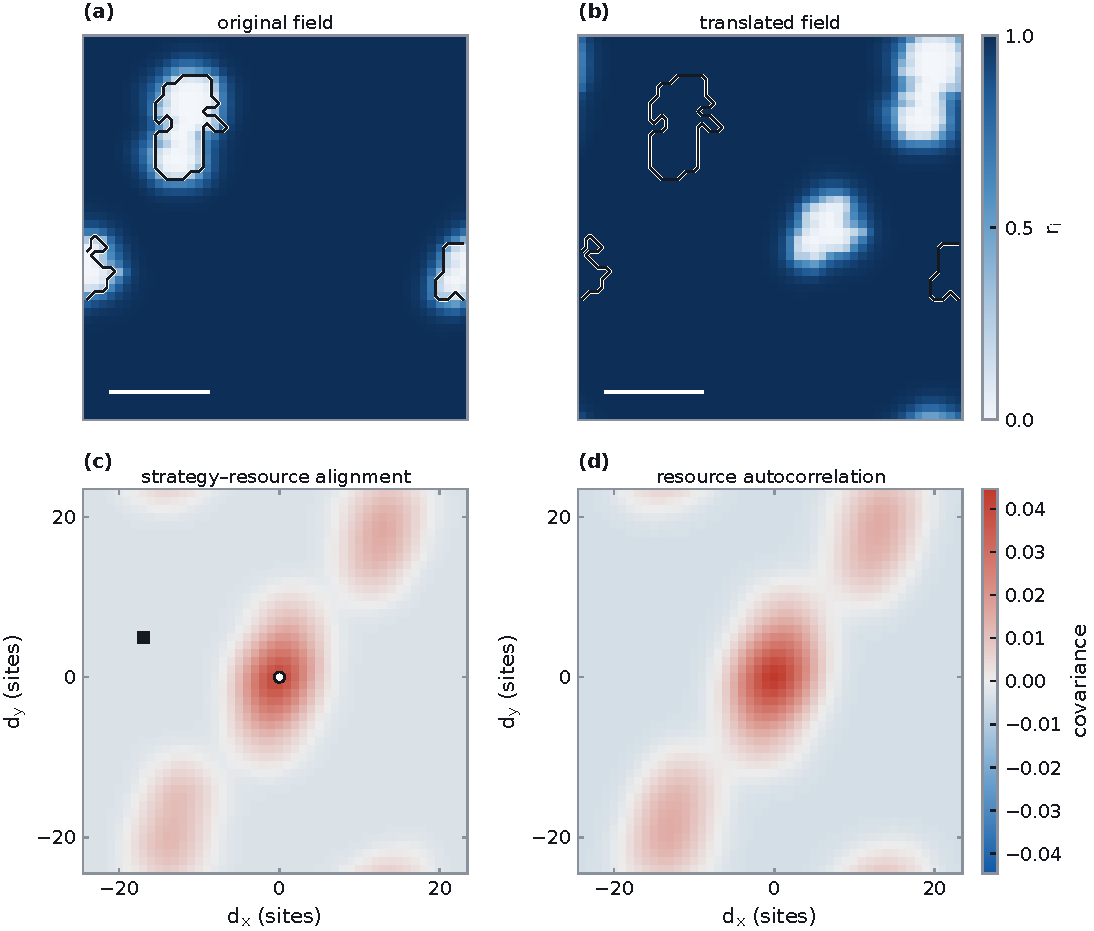
\includegraphics[width=0.83\textwidth]{fig02_interventions.pdf}
\caption{Controlled change in relative strategy--resource alignment. (a,b) Original resource field and the same field translated by $(5,-17)$ sites, with the strategy boundary unchanged. Scale bars represent 12 sites. (c) Strategy--resource cross-covariance $C_{sr}(\mathbf d)$ across periodic translations; the circle and square mark the fields in (a,b). (d) Resource autocorrelation $\Gamma_r(\mathbf d)$, which is invariant under the translation. The covariance maps use a common signed color scale. These panels characterize spatial organization, not collapse probability.}
\label{fig:alignment}
\end{figure*}


For a grown configuration $X$ in which neither event has occurred, let $\tau_A$ and $\tau_B$ be the first recovery and collapse confirmation times measured from the continuation origin. The conditional fate probabilities at horizon $H$ are
\begin{equation}
\label{eq:conditional_fate}
\begin{aligned}
q_B(H\mid X)&=\Pr(\tau_B\le H,\ \tau_B<\tau_A\mid X),\\
q_A(H\mid X)&=\Pr(\tau_A\le H,\ \tau_A<\tau_B\mid X),\\
q_U(H\mid X)&=1-q_A(H\mid X)-q_B(H\mid X).
\end{aligned}
\end{equation}
We compare these probabilities after a single resource translation of each grown configuration. Both fields then evolve under the original dynamics, retaining the same strategy state at the start of each continuation.

\begin{table}[t]
\caption{Translation-induced changes in conditional collapse probability at $H=40000$ MCS. The comparison uses 48 configurations at their first 5\% defector crossing, with 16 fresh continuations per field and direction. Four directions are averaged within each magnitude; 95\% bootstrap intervals retain pairing within configurations.}
\label{tab:translation_risk}
\centering
\begin{tabular}{lrr}
\toprule
Comparison & $\Delta q_B$ & 95\% interval \\
\midrule
Short shift--original & $0.0498$ & $[0.0052,0.0944]$ \\
Long shift--original & $-0.0628$ & $[-0.0983,-0.0273]$ \\
Long--short shift & $-0.1126$ & $[-0.1370,-0.0882]$ \\
\bottomrule
\end{tabular}
\end{table}

Despite these invariants, the translated configurations have different finite-time collapse probabilities. A short translation increases the conditional probability of collapse relative to the original field, whereas a longer translation decreases it. In the paired continuation experiment at $H=40\,000$ MCS, the changes are $+0.0498$ and $-0.0628$, respectively (Table~\ref{tab:translation_risk}). An independent displacement-length series also shows a turnover rather than a monotonic dependence on translation magnitude. Thus the relative arrangement of the two fields affects the outcome even when the strategy pattern and the single-field resource statistics are held fixed. Displacement vectors, sampling details, and uncertainty estimates are given in Sec.~\ref{sm-sec:checks} of the Supplemental Material.

The interfacial resource profiles in Fig.~\ref{fig:resourcelayers} provide a local view of this effect. Distance is measured relative to the strategy boundary, with negative values inside defector regions and positive values inside cooperative regions. Before translation, the mean resource profile rises sharply across the interface. A short shift broadens this transition, whereas the displayed long shift moves resource-rich regions toward parts of the boundary and raises resource levels at neighboring cooperative sites.


\begin{figure*}[tp]
\centering
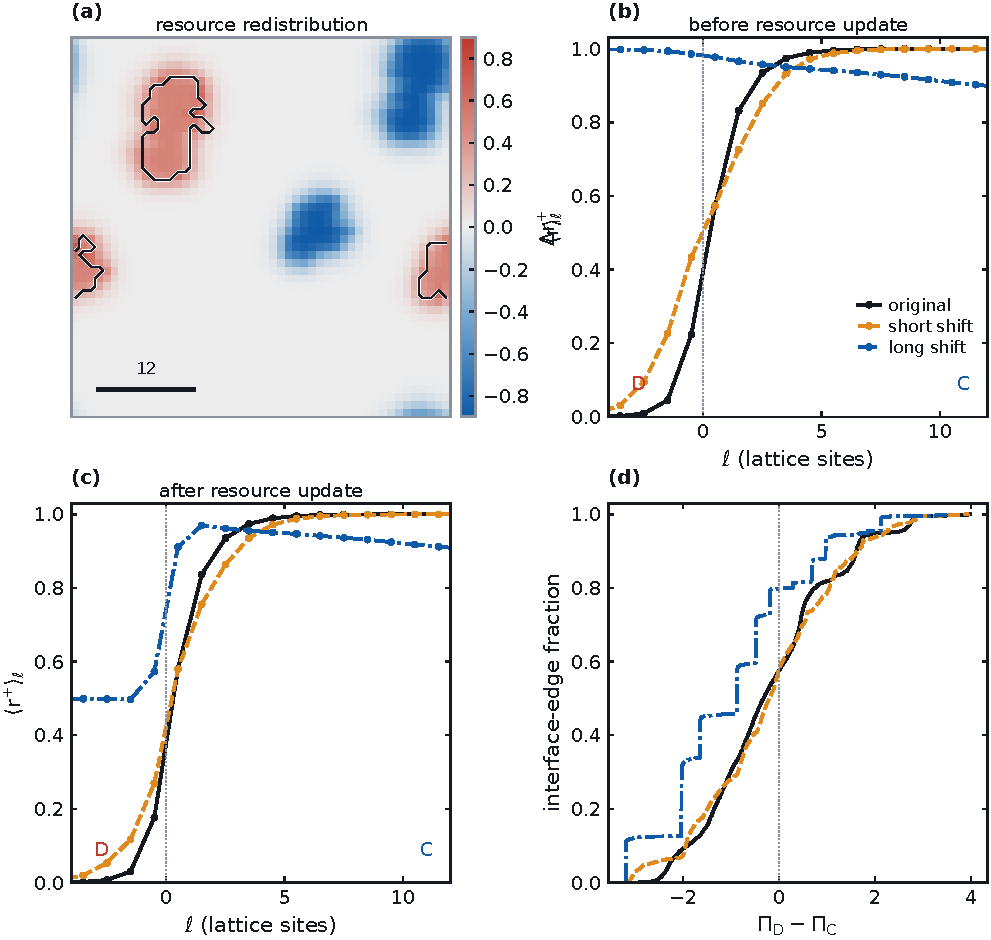
\includegraphics[width=0.8\textwidth]{fig10_resource_layers.pdf}
\caption{Resource profiles and payoff gaps near a fixed strategy boundary. (a) Difference in the post-update resource field under the displayed long translation, with the strategy interface unchanged (scale bar: 12 sites). (b,c) Mean resource profiles before and after one resource update, plotted against signed periodic graph distance $\ell$ from the interface. Negative and positive distances lie in defector and cooperator regions, respectively, with boundary sites at $\ell=\pm1/2$. (d) Cumulative distribution of interfacial payoff gaps after the resource update. The displayed short and long translations are $(2,1)$ and $(5,-17)$. Profiles pool lattice sites from 48 configurations within each distance shell; gap distributions pool undirected cooperator--defector edges. Only the displayed displacement vectors are used in these panels, without rotation averaging.}
\label{fig:resourcelayers}
\end{figure*}


Renewal, depletion, and diffusion subsequently act on the translated field, but a single update does not remove the change in boundary conditions. For the displayed long shift, the interfacial payoff-gap distribution shifts toward values favoring cooperation. Relative field alignment therefore changes the immediate microscopic bias of interface motion. Its effect on collapse probability also depends on how the interface and resource layer evolve after this initial perturbation.

Alignment also affects net resource production through the strategy--resource covariance. Subtracting Eq.~\eqref{eq:balance} for original and translated fields with equal initial strategy and resource means gives
\begin{equation}
\label{eq:translation_balance}
\Delta\bar r(1)=(\delta-g)\Delta C_{sr}(0).
\end{equation}
Equation~\eqref{eq:translation_balance} shows that changing relative alignment alters the next mean-resource increment even though the initial resource total is unchanged. Interfacial payoff differences and total resource production thus respond to the same spatial rearrangement through distinct local and global mechanisms. Neither response can be inferred from the initial mean resource alone.
